%%%%%%%%%%%%%%%%%%%%%%%%%%%%%%%%%%%%%
%                                   %
% Compile with XeLaTeX and biber    %
%                                   %
% Questions or comments:            %
%                                   %
% joshua dot mcneill at uga dot edu %
%                                   %
%%%%%%%%%%%%%%%%%%%%%%%%%%%%%%%%%%%%%

\documentclass{beamer}
  % Read in standard preamble (cosmetic stuff)
  %%%%%%%%%%%%%%%%%%%%%%%%%%%%%%%%%%%%%%%%%%%%%%%%%%%%%%%%%%%%%%%%
% This is a standard preamble used in for all slide documents. %
% It basically contains cosmetic settings.                     %
%                                                              %
% Joshua McNeill                                               %
% joshua dot mcneill at uga dot edu                            %
%%%%%%%%%%%%%%%%%%%%%%%%%%%%%%%%%%%%%%%%%%%%%%%%%%%%%%%%%%%%%%%%

% Beamer settings
% \usetheme{Berkeley}
\usetheme{CambridgeUS}
% \usecolortheme{dove}
% \usecolortheme{rose}
\usecolortheme{seagull}
\usefonttheme{professionalfonts}
\usefonttheme{serif}
\setbeamertemplate{bibliography item}{}

% Packages and settings
\usepackage{fontspec}
  \setmainfont{Charis SIL}
\usepackage{hyperref}
  \hypersetup{colorlinks=true,
              allcolors=blue}
\usepackage{graphicx}
  \graphicspath{{../../figures/}}
\usepackage[normalem]{ulem}
\usepackage{enumerate}

% Document information
\author{M. McNeill}
\title[FREN2001]{Français 2001}
\institute{\url{joshua.mcneill@uga.edu}}
\date{}

%% Custom commands
% Lexical items
\newcommand{\lexi}[1]{\textit{#1}}
% Gloss
\newcommand{\gloss}[1]{`#1'}
\newcommand{\tinygloss}[1]{{\tiny`#1'}}
% Orthographic representations
\newcommand{\orth}[1]{$\langle$#1$\rangle$}
% Utterances (pragmatics)
\newcommand{\uttr}[1]{`#1'}
% Sentences (pragmatics)
\newcommand{\sent}[1]{\textit{#1}}
% Base dir for definitions
\newcommand{\defs}{../definitions}


  % Packages and settings

  % Document information
  \subtitle[Habitudes et imparfait]{Les habitudes et l'imparfait}

\begin{document}
  % Read in the standard intro slides (title page and table of contents)
  \begin{frame}
    \titlepage
    \tiny{Office: % Basically a variable for office hours location
Gilbert 121\\
          Office hours: % Basically a variable for office hours
 lundi, mercredi, vendredi 10:10--11:10
}
  \end{frame}

  \begin{frame}{Imparfait encore}
    \begin{center}
      \begin{tabular}{l | l l | l l}
  \multicolumn{5}{c}{parler $\to$ parlons $\to$ parl-} \\
      & \multicolumn{2}{l |}{singulier} & \multicolumn{2}{l}{pluriel} \\
  \hline
  1re & je         & parlais            & nous        & parlions \\
  2e  & tu         & parlais            & vous        & parliez \\
  \hline
  3e  & il (masc)  &                    & ils (masc)  & \\
      & elle (fem) & parlait            & elles (fem) & parlaient \\
      & on         &                    &             & \\
\end{tabular}

    \end{center}
    D'habitude, c'est pour décrire des situations au passé.
  \end{frame}

  \begin{frame}{Imparfait irregulier}
    \begin{center}
      \input{../conj_tables/être_imp.tex}
    \end{center}
  \end{frame}

  \begin{frame}{Une histoire}
    \begin{columns}
      \scriptsize
      \column{0.5\textwidth}
        Finissons l'histoire ensemble...
        \begin{enumerate}
          \item \underline{\uncover<2->{C'était}} (ce / être) le mois de juin.
          \item<3-> Des enfants \underline{\uncover<4->{jouaient}} (jouer) dans le jardin.
          \item<5-> Le père \underline{\uncover<6->{parlait}} (parler) avec sa fille lorsque un ballon l'a frappé.
          \item<7-> Son fils \underline{\uncover<8->{jouait}} (jouer) au foot.
          \item<9-> La mère et la tante des enfants \underline{\uncover<10->{buvaient}} (boire) un jus d'orange, donc elles ne l'ont pas regardé.
          \item<11-> Ces femmes \underline{\uncover<12->{ne regardaient pas}} (ne pas regarder) les enfants.
          \item<13-> Leur frère \underline{\uncover<14->{préparait}} (préparer) un repas.
          \item<15-> Le chien et le chat \underline{\uncover<16->{dormaient}} (dormir), mais ils ont été réveillés par l'odeur.
        \end{enumerate}
      \column{0.5\textwidth}
        \begin{minipage}[0.6\textheight]{\linewidth}
          \begin{center}
            \only<3-4>{
              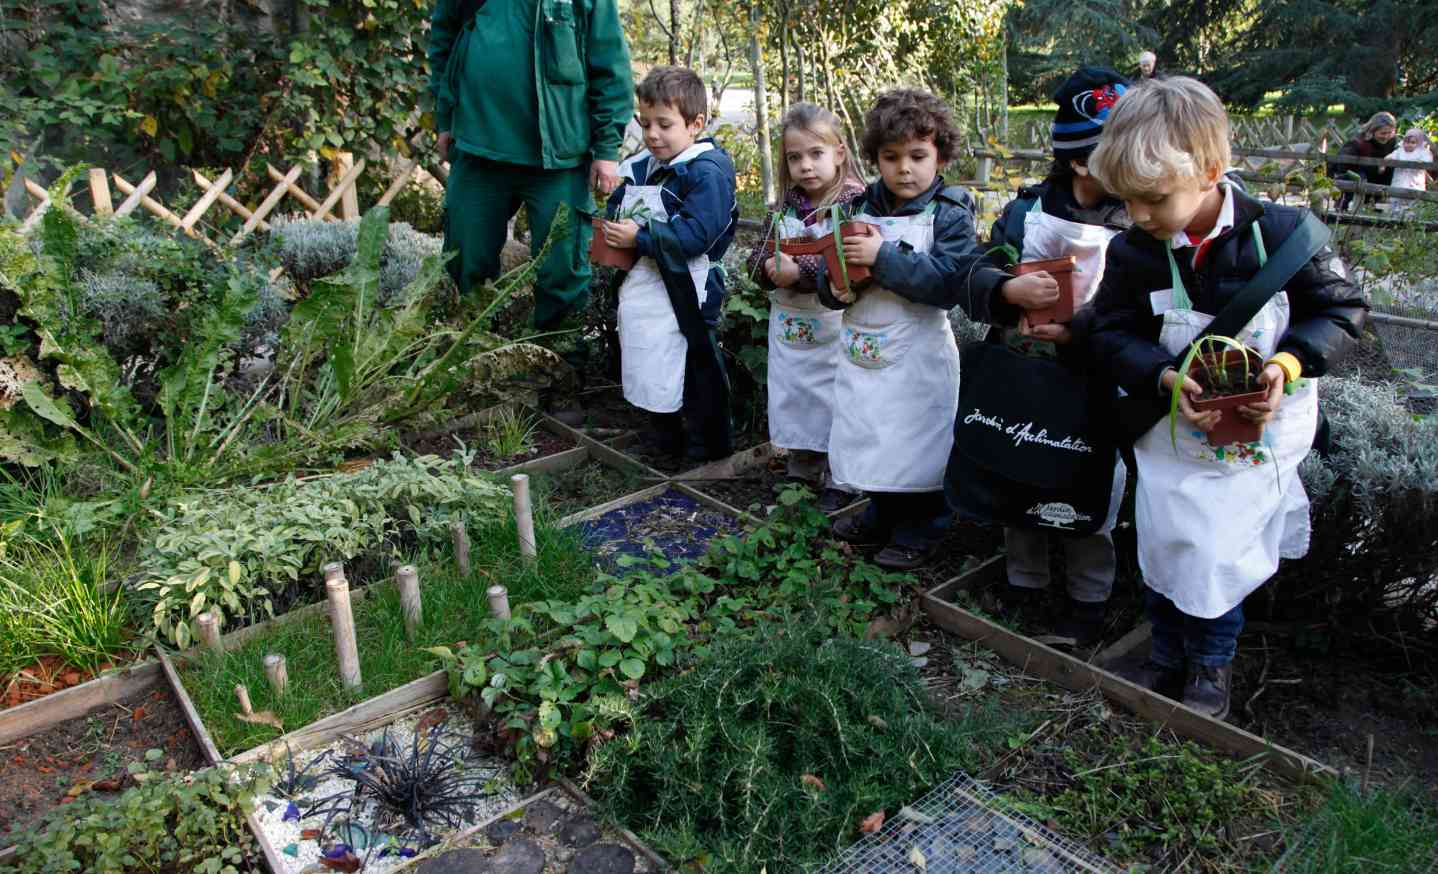
\includegraphics[scale=0.15]{jardin.jpg}
            }
            \only<5-6>{
              
\includegraphics[scale=0.25]{ballon.jpg} \\
              Marouane Fellaini de la Belgique
            }
            \only<7-8>{
              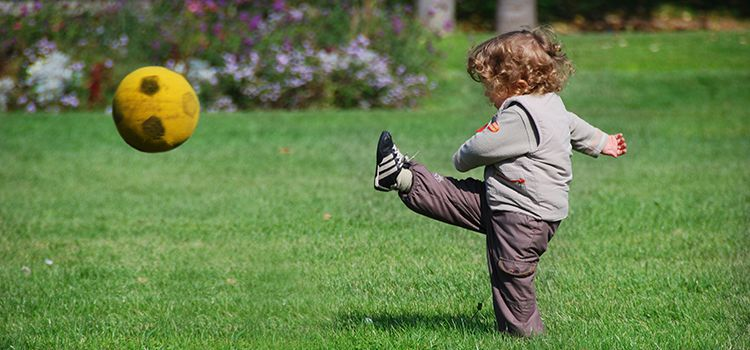
\includegraphics[scale=0.9]{enfant_foot.jpg}
            }
            \only<9-12>{
              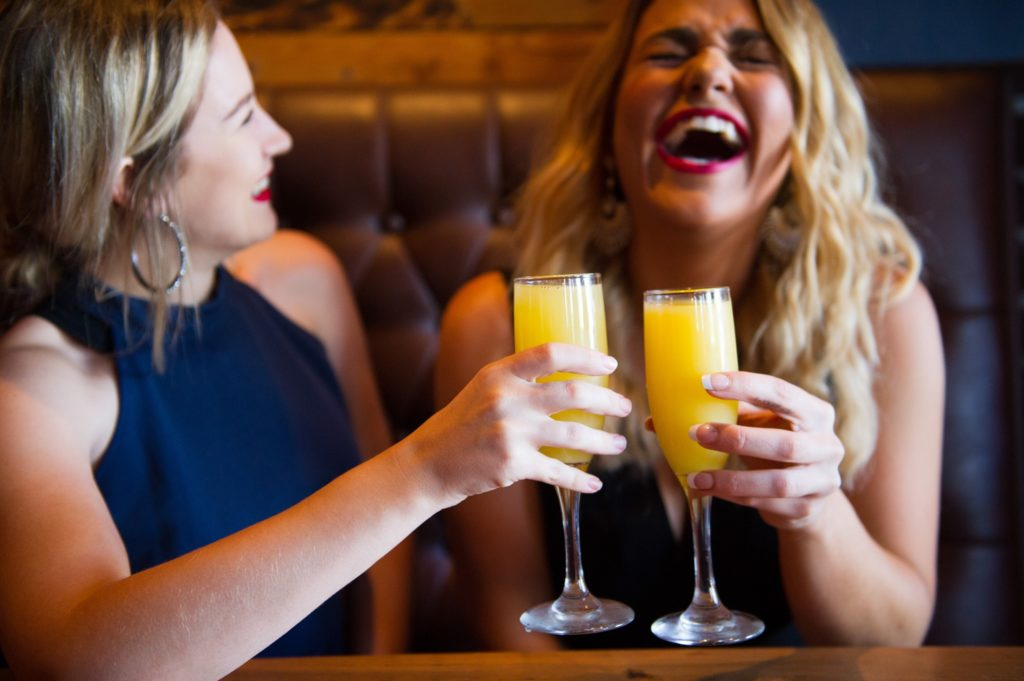
\includegraphics[scale=0.16]{mimosas.jpg}
            }
            \only<13-14>{
              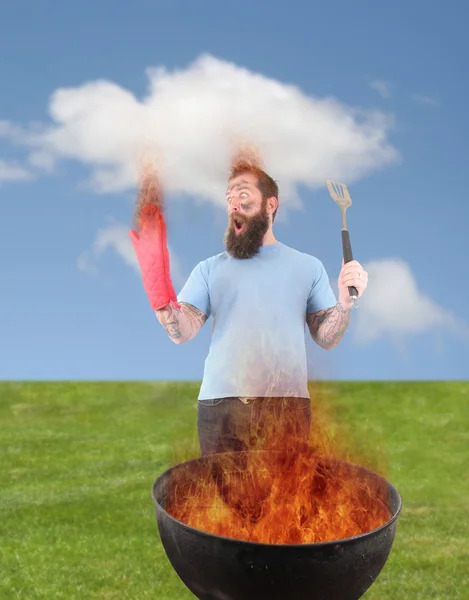
\includegraphics[scale=0.28]{bbq.jpg}
            }
            \only<15-16>{
              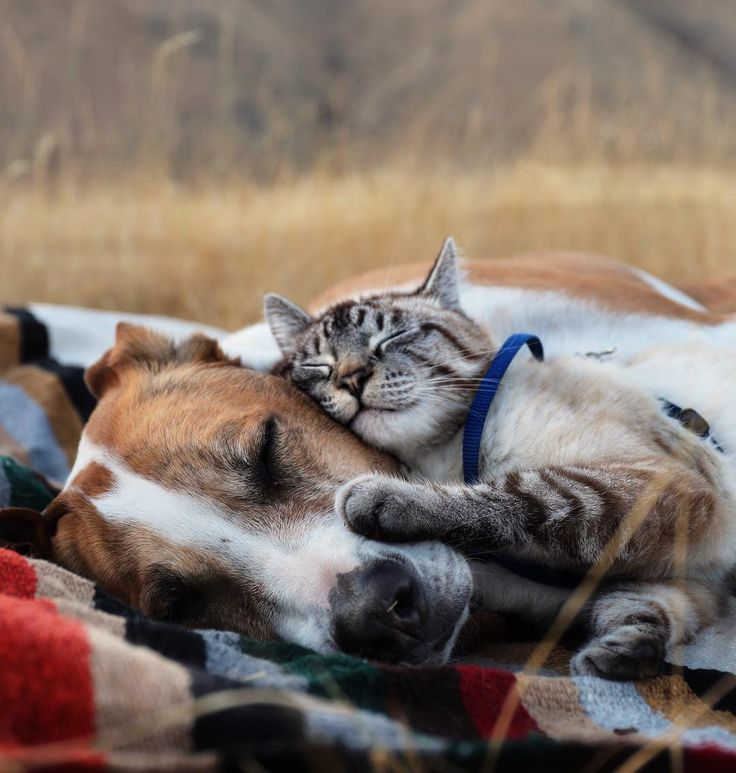
\includegraphics[scale=0.19]{chien_chat.jpg}
            }
          \end{center}
        \end{minipage}
    \end{columns}
  \end{frame}

  \begin{frame}{}
    \begin{center}
      \Large Quiz
    \end{center}
  \end{frame}

  \begin{frame}{Ton enfance}
    Pose des questions à un/e partenaire au sujet de son enfance \gloss{childhood}.
    Utilise l'imparfait le cas échéant \gloss{where appropriate}.
    \begin{description}
      \item[\textbf{Modèle:}] \textit{habiter ici}
      \item[E1:] Est-ce que tu habitais ici pendant ton enfance?
      \item[E2:] Non, j'habitais à Chicago avec mes parents.
    \end{description}
    \begin{columns}[t]
      \column{0.5\textwidth}
        \begin{enumerate}
          \item habiter ici
          \item avoir des animaux
          \item aimer aller à l'école
          \item faire du sport
        \end{enumerate}
      \column{0.5\textwidth}
        \begin{enumerate}
          \setcounter{enumi}{4}
          \item jouer d'un instrument
          \item aller souvent chez des amis
          \item partir souvent en vacances
          \item avoir une résidence secondaire
        \end{enumerate}
    \end{columns}
  \end{frame}

  \begin{frame}{}
    \begin{center}
      \Large Questions?
    \end{center}
  \end{frame}
\end{document}
